% =====================================================================
\chapter{The Schwarzschild metric}\label{ch:schwarzschild}
% =====================================================================

The Schwarzschild solution describes the gravitational field outside a spherically symmetric body, such as the Earth or the Sun (to a very good approximation). It is the simplest and most important exact solution of the EFE.

\section{Assumptions and the form of the metric}

We are looking for a solution of the EFE:
\begin{enumerate}[label=\arabic*),start=0,nosep]
\item in \textbf{vacuum}, $T_{\mu\nu}=0\Rightarrow G_{\mu\nu}=0$;
\item in $(1+3)$ dimensions, working with the $(+,-,-,-)$ metric;
\item \textbf{spherically symmetric};
\item \textbf{static}.
\end{enumerate}
We work in ``spherical coordinates'' $(t,r,\theta,\phi)$ (Schwarzschild coordinates).

\paragraph{The metric is diagonal.} From requirements 2) and 3), the metric must be invariant under the discrete transformations
\begin{align*}
  (t,r,\theta,\phi)&\to(-t,r,\theta,\phi)\quad\text{(static: time reversal)},\\
  (t,r,\theta,\phi)&\to(t,r,-\theta,\phi)\quad\text{(spherical symmetry: reflection)},\\
  (t,r,\theta,\phi)&\to(t,r,\theta,-\phi)\quad\text{(spherical symmetry: reflection)},
\end{align*}
i.e.\ $g'_{\mu\nu}(x)=g_{\mu\nu}(x)$. But $g_{\mu\nu}$ is a $(0,2)$ tensor, $g'_{\mu\nu}=\frac{\pd x^\alpha}{\pd x'^\mu}\frac{\pd x^\beta}{\pd x'^\nu}g_{\alpha\beta}$. Consider $t\to-t$: the only non-trivial Jacobian element is $\pd t/\pd t'=-1$, so
\[
  g'_{00}=\frac{\pd x^\alpha}{\pd(-t)}\frac{\pd x^\beta}{\pd(-t)}g_{\alpha\beta}=g_{00},\qquad
  g'_{0r}=\frac{\pd x^\alpha}{\pd(-t)}\frac{\pd x^\beta}{\pd r}g_{\alpha\beta}=-g_{0r},\qquad g'_{0\nu}=-g_{0\nu}\ \ (\nu\neq0).
\]
The static condition requires $g'_{0\nu}=g_{0\nu}$, hence $g_{0\nu}=0$ for all $\nu\neq0$. Working similarly with the other two reflections, $g_{2\nu}=0$ for $\nu\neq2$ and $g_{3\nu}=0$ for $\nu\neq3$. Gathering things: $g_{\mu\nu}=0$ for all $\mu\neq\nu$: \textbf{the metric is diagonal} (in this coordinate system).

\paragraph{Spherical symmetry.}
\begin{enumerate}[label=(\roman*),nosep]
\item On each radial line ($\theta,\phi=$ const), $g_{rr}$ and $g_{tt}$ can only depend on $r$ (not on $t$, due to the static condition).
\item On the hypersurfaces $t,r=\text{const}$ the metric should take the form of that of a 2-sphere.
\end{enumerate}
Therefore
\[
  c^2\dd\tau^2=A(r)\dd t^2-B(r)\dd r^2-D(r)\,r^2\big(\dd\theta^2+\sin^2\theta\,\dd\phi^2\big).
\]
$D(r)$ can be eliminated by a coordinate transformation $r\to R(r)$ such that $R^2=D(r)r^2$ (this redefines $A$ and $B$); for simplicity we keep denoting the new radial coordinate by $r$:
\begin{equation}
  c^2\dd\tau^2=A(r)\dd t^2-B(r)\dd r^2-r^2\big(\dd\theta^2+\sin^2\theta\,\dd\phi^2\big).
  \label{eq:schw-ansatz}
\end{equation}
We now want to determine $A(r)$ and $B(r)$. Note that, because $\dd t$ and $\dd r$ are multiplied by functions, $t$ and $r$ are not, in general, proper time and proper distance.

\section{Solving the Einstein equations}

\paragraph{Vacuum equations.} Note that
\[
  G_{\mu\nu}=0\ \Rightarrow\ g^{\mu\nu}G_{\mu\nu}=g^{\mu\nu}\Big(R_{\mu\nu}-\frac12g_{\mu\nu}R\Big)=R-2R=-R=0\ \Rightarrow\ R=0 ,
\]
so $G_{\mu\nu}=0$ reduces to $\boxed{R_{\mu\nu}=0}$. Manifolds satisfying this are called \textbf{Ricci-flat}. The steps to solve the equations are:
\begin{enumerate}[nosep]
\item compute the $\Gamma$'s;
\item compute $\Riem{\mu}{\nu}{\rho}{\sigma}$ (actually not needed, see below);
\item compute $R_{\mu\nu}$;
\item solve $R_{\mu\nu}=0$.
\end{enumerate}

\subsection{Christoffel symbols: the Lagrangian trick}
How to compute the $\Gamma$'s? (i) Brute force, from \eqref{eq:christoffel} (a good exercise, but tedious); or (ii) use the trick: the Lagrangian
\[
  \mathcal L=\frac12g_{\mu\nu}\frac{\dd x^\mu}{\dd\tau}\frac{\dd x^\nu}{\dd\tau}
\]
and the Euler--Lagrange equations $\frac{\dd}{\dd\tau}\big(\frac{\pd\mathcal L}{\pd\dot x^\alpha}\big)-\frac{\pd\mathcal L}{\pd x^\alpha}=0$ ($\dot{}\equiv\dd/\dd\tau$) give the geodesic equations, from which the $\Gamma$'s can be read off.

\textit{Proof.} Since the metric only depends on the position and not on the velocities (in analytical mechanics positions and velocities are independent coordinates),
\begin{align*}
  0&=\frac{\dd}{\dd\tau}\left[\frac{\pd}{\pd\dot x^\alpha}\Big(\frac12g_{\mu\nu}\dot x^\mu\dot x^\nu\Big)\right]-\frac{\pd}{\pd x^\alpha}\Big(\frac12g_{\mu\nu}\dot x^\mu\dot x^\nu\Big)
   =\frac{\dd}{\dd\tau}\left[\frac12g_{\mu\nu}\big(\delta^\mu{}_\alpha\dot x^\nu+\dot x^\mu\delta^\nu{}_\alpha\big)\right]-\frac12\frac{\pd g_{\mu\nu}}{\pd x^\alpha}\dot x^\mu\dot x^\nu\\
  &=\frac{\dd}{\dd\tau}\big[g_{\alpha\mu}\dot x^\mu\big]-\frac12\pd_\alpha g_{\mu\nu}\dot x^\mu\dot x^\nu
   =g_{\alpha\mu}\ddot x^\mu+\pd_\nu g_{\alpha\mu}\dot x^\nu\dot x^\mu-\frac12\pd_\alpha g_{\mu\nu}\dot x^\mu\dot x^\nu\\
  &=g_{\alpha\mu}\ddot x^\mu+\frac12\big(\pd_\nu g_{\mu\alpha}+\pd_\mu g_{\nu\alpha}-\pd_\alpha g_{\mu\nu}\big)\dot x^\mu\dot x^\nu .
\end{align*}
Multiplying by $g^{\rho\alpha}$: $\ddot x^\rho+\Ga{\rho}{\mu}{\nu}\dot x^\mu\dot x^\nu=0$. $\blacksquare$

\emph{The method:} bring each Euler--Lagrange equation to the form $\ddot x^\rho+(\text{stuff})\,\dot x\dot x=0$ and read the Christoffel symbols directly. Be careful with factors $\frac12$: a crossed term $\dot x^\mu\dot x^\nu$ with $\mu\neq\nu$ appears twice in the sum ($\Ga{\rho}{\mu}{\nu}+\Ga{\rho}{\nu}{\mu}=2\Ga{\rho}{\mu}{\nu}$), so its coefficient is $2\Ga{\rho}{\mu}{\nu}$.

For \eqref{eq:schw-ansatz}, $\mathcal L=\frac12\big(A\dot t^2-B\dot r^2-r^2\dot\theta^2-r^2\sin^2\theta\,\dot\phi^2\big)$, with $'\equiv\dd/\dd r$:
\begin{itemize}
\item $t$: $\frac{\dd}{\dd\tau}(A\dot t)=0\Rightarrow A\ddot t+A'\dot r\dot t=0\Rightarrow\ddot t+\frac{A'}{A}\dot t\dot r=0$, so $2\Ga{t}{t}{r}=A'/A$.
\item $r$: $\frac{\dd}{\dd\tau}(-B\dot r)-\frac12\big(A'\dot t^2-B'\dot r^2-2r\dot\theta^2-2r\sin^2\theta\dot\phi^2\big)=0$, i.e.
\[
  \ddot r+\frac{A'}{2B}\dot t^2+\frac{B'}{2B}\dot r^2-\frac rB\dot\theta^2-\frac{r\sin^2\theta}{B}\dot\phi^2=0 .
\]
\item $\theta$: $\frac{\dd}{\dd\tau}(-r^2\dot\theta)+r^2\sin\theta\cos\theta\,\dot\phi^2=0\Rightarrow\ddot\theta+\frac2r\dot r\dot\theta-\sin\theta\cos\theta\,\dot\phi^2=0$.
\item $\phi$: $\frac{\dd}{\dd\tau}(-r^2\sin^2\theta\,\dot\phi)=0\Rightarrow\ddot\phi+\frac2r\dot r\dot\phi+2\cot\theta\,\dot\theta\dot\phi=0$.
\end{itemize}
Reading off the coefficients:
\begin{keyresult}[Christoffel symbols of the static spherically symmetric metric]
\begin{gather*}
  \Ga{t}{t}{r}=\Ga{t}{r}{t}=\frac{A'}{2A},\qquad
  \Ga{r}{t}{t}=\frac{A'}{2B},\qquad\Ga{r}{r}{r}=\frac{B'}{2B},\qquad\Ga{r}{\theta}{\theta}=-\frac rB,\qquad\Ga{r}{\phi}{\phi}=-\frac{r\sin^2\theta}{B},\\
  \Ga{\theta}{r}{\theta}=\Ga{\theta}{\theta}{r}=\frac1r,\qquad\Ga{\theta}{\phi}{\phi}=-\sin\theta\cos\theta,\qquad
  \Ga{\phi}{r}{\phi}=\Ga{\phi}{\phi}{r}=\frac1r,\qquad\Ga{\phi}{\theta}{\phi}=\Ga{\phi}{\phi}{\theta}=\cot\theta,
\end{gather*}
and the remaining $\Gamma$'s ($64-13=51$ of them) vanish.
\end{keyresult}

\subsection{The Ricci tensor}
We do not need the entire Riemann tensor, because we actually look for the Ricci tensor. Trick: compute $R_{\mu\nu}$ directly from the $\Gamma$'s,
\begin{equation}
  R_{\mu\nu}=\Riem{\lambda}{\mu}{\lambda}{\nu}=\pd_\lambda\Ga{\lambda}{\mu}{\nu}-\pd_\nu\Ga{\lambda}{\mu}{\lambda}+\Ga{\lambda}{\lambda}{\rho}\Ga{\rho}{\mu}{\nu}-\Ga{\lambda}{\nu}{\rho}\Ga{\rho}{\mu}{\lambda}.
  \label{eq:ricci-from-gamma}
\end{equation}

\begin{example}{Computation of $R_{\theta\theta}$}{Rthth}
\begin{itemize}[nosep]
\item $\pd_\lambda\Ga{\lambda}{\theta}{\theta}=\pd_r\big(-\frac rB\big)=-\frac1B+\frac{rB'}{B^2}$;
\item $-\pd_\theta\Ga{\lambda}{\theta}{\lambda}=-\pd_\theta\cot\theta=\frac{1}{\sin^2\theta}$;
\item $\Ga{\lambda}{\lambda}{r}\Ga{r}{\theta}{\theta}=\Big(\frac{A'}{2A}+\frac{B'}{2B}+\frac2r\Big)\Big(-\frac rB\Big)=-\frac{rA'}{2AB}-\frac{rB'}{2B^2}-\frac2B$;
\item $-\Ga{\lambda}{\theta}{\rho}\Ga{\rho}{\theta}{\lambda}=-\big(\Ga{r}{\theta}{\theta}\Ga{\theta}{\theta}{r}+\Ga{\theta}{\theta}{r}\Ga{r}{\theta}{\theta}+\Ga{\phi}{\theta}{\phi}\Ga{\phi}{\theta}{\phi}\big)=\frac2B-\cot^2\theta$.
\end{itemize}
Summing, and using $\frac1{\sin^2\theta}-\cot^2\theta=1$:
\[
  R_{\theta\theta}=\frac{B-1}{B}-\frac{rA'}{2AB}+\frac{rB'}{2B^2}.
\]
\end{example}
Proceeding in the same way for the other components (``4 pages later, whichever method one follows\dots'') one finds that the only non-vanishing components are
\begin{align}
  R_{tt}&=\frac{A''}{2B}+\frac{A'}{rB}-\frac{(A')^2}{4AB}-\frac{A'B'}{4B^2},\nonumber\\
  R_{rr}&=-\frac{A''}{2A}+\frac{B'}{rB}+\frac{(A')^2}{4A^2}+\frac{A'B'}{4AB},\nonumber\\
  R_{\theta\theta}&=\frac{B-1}{B}-\frac{rA'}{2AB}+\frac{rB'}{2B^2},\qquad R_{\phi\phi}=\sin^2\theta\,R_{\theta\theta}.
  \label{eq:ricci-static}
\end{align}
It is convenient to raise one index ($R^\mu{}_\nu=g^{\mu\alpha}R_{\alpha\nu}$, with $g^{tt}=1/A$, $g^{rr}=-1/B$, $g^{\theta\theta}=-1/r^2$):
\begin{align}
  R^t{}_t&=\frac{A''}{2AB}-\frac{A'B'}{4AB^2}-\frac{(A')^2}{4A^2B}+\frac{A'}{rAB},\nonumber\\
  R^r{}_r&=\frac{A''}{2AB}-\frac{A'B'}{4AB^2}-\frac{(A')^2}{4A^2B}-\frac{B'}{rB^2},\nonumber\\
  R^\theta{}_\theta&=R^\phi{}_\phi=\frac{A'}{2rAB}-\frac{B'}{2rB^2}-\frac{B-1}{r^2B}.
\end{align}

\subsection{Solving $R^\mu{}_\nu=0$}
\textbf{Observation 1:} the combination $R^t{}_t-R^r{}_r-R^\theta{}_\theta-R^\phi{}_\phi$ does \emph{not} contain $A$:
\[
  R^t{}_t-R^r{}_r-2R^\theta{}_\theta=\frac{A'}{rAB}+\frac{B'}{rB^2}-\frac{A'}{rAB}+\frac{B'}{rB^2}+\frac{2(B-1)}{r^2B}=\frac{2B'}{rB^2}+\frac{2(B-1)}{r^2B}.
\]
\textbf{Observation 2:} $R^\mu{}_\nu=0$ must hold for all $\mu,\nu$, so every combination vanishes too. From these observations:
\begin{itemize}
\item $R^t{}_t-R^r{}_r-2R^\theta{}_\theta=0\Rightarrow\frac{2B'}{rB^2}+\frac{2(B-1)}{r^2B}=0\Rightarrow\frac{\dd B}{B(B-1)}+\frac{\dd r}{r}=0$. Integrating, with $\frac{1}{B(B-1)}=\frac1{B-1}-\frac1B$: $\ln\frac{B-1}{B}=-\ln r+\text{const}$, i.e.\ $1-\frac1B=\frac ar$:
\begin{equation}
  B(r)=\Big(1-\frac ar\Big)^{-1},
\end{equation}
where $a$ is an integration constant.
\item $R^t{}_t-R^r{}_r=0\Rightarrow\frac{A'}{rAB}+\frac{B'}{rB^2}=0\Rightarrow\frac{\dd A}{A}+\frac{\dd B}{B}=0\Rightarrow AB=\text{const}$.
\end{itemize}
(One checks that the remaining equation, $R^\theta{}_\theta=0$, is then automatically satisfied.) Now, to fix the constants, we have to impose the boundary conditions. If the metric is to describe the space-time around a spherically symmetric, static object, it must become flat far away:
\[
  A(r)\to c^2,\quad B(r)\to1\qquad\text{as }r\to\infty\qquad\Longrightarrow\qquad g_{\mu\nu}\to\eta_{\mu\nu}.
\]
$B\to1$ is automatically satisfied; $AB=\text{const}=c^2$ gives $A(r)=c^2(1-a/r)$. Finally, the metric must reproduce the Newtonian limit, $g_{00}=1+2\Phi/c^2$ with $x^0=ct$, i.e.\ $A=c^2(1+2\Phi/c^2)$, with $\Phi=-\GN M/r$. Hence $a=2\GN M/c^2$.

\begin{keyresult}[The Schwarzschild metric]
\begin{equation}
  c^2\dd\tau^2=\Big(1-\frac{2\GN M}{c^2r}\Big)c^2\dd t^2-\Big(1-\frac{2\GN M}{c^2r}\Big)^{-1}\dd r^2-r^2\dd\Omega^2 ,\qquad \dd\Omega^2=\dd\theta^2+\sin^2\theta\,\dd\phi^2,
  \label{eq:schwarzschild}
\end{equation}
with the \textbf{Schwarzschild radius}
\begin{equation}
  \rs\equiv\frac{2\GN M}{c^2}.
\end{equation}
\end{keyresult}

\section{Remarks}

\begin{enumerate}
\item \textbf{Birkhoff's theorem:} any spherically symmetric solution of the vacuum EFE is necessarily static (and is therefore Schwarzschild). Hence the exterior of a spherically symmetric pulsating or collapsing star is still described by \eqref{eq:schwarzschild}: spherically symmetric oscillations do not emit gravitational waves.
\item The Schwarzschild metric appears to have \textbf{two singularities}: at $r=0$ (where $g_{tt}\to\infty$; this one is impossible to remove, see \cref{ch:blackholes}) and at $r=\rs$ (where $g_{rr}\to\infty$).
\item For ordinary objects the singularity at $r=\rs$ is irrelevant, e.g.
\begin{itemize}[nosep]
\item Earth: $R_\oplus\simeq6400$\,km, $r_s^\oplus\simeq0.9$\,cm;
\item Sun: $R_\odot\simeq7\times10^5$\,km, $r_s^\odot\simeq3$\,km.
\end{itemize}
$r_s$ lies inside the object, where there is no vacuum, so the Schwarzschild metric does not apply there (one needs an interior solution, see Problem Sheet 4). However, for really massive and compact objects, $r_s$ lies outside the object itself (in vacuum): then it is relevant. When $r\sim\rs$: black holes.
\item For $r<\rs$ the signs of $g_{tt}$ and $g_{rr}$ flip: the $t$-like component of the metric becomes space-like and $r$ becomes time-like (inside, $r$ plays the role of time and inevitably decreases).
\end{enumerate}

\paragraph{Interpretation of the Schwarzschild coordinates.}
\begin{itemize}
\item $\theta,\phi$: standard angles on the spheres of symmetry.
\item $r$: it is \emph{not} the proper radial distance (that would be $\int\sqrt{B}\,\dd r$). It has a geometric interpretation: the sphere $r=$ const, $t=$ const has proper area $4\pi r^2$ (``areal radius''), as the induced metric is $r^2\dd\Omega^2$.
\item $t$: fair enough, it is the proper time of a static observer at $r\to\infty$, where the metric is flat. A static observer at radius $r$ ($\dd r=\dd\theta=\dd\phi=0$) measures the proper time $\dd\tau=\sqrt{1-\rs/r}\,\dd t<\dd t$.
\end{itemize}
\textit{Consequence (gravitational redshift revisited).} Since the metric is static, the coordinate-time interval between two wave crests is the same at emission and at reception. A photon emitted at $r_e$ with frequency $f_e$ (measured by a static emitter) and received by a static observer at $r_o$ has
\begin{equation}
  \frac{f_o}{f_e}=\frac{\dd\tau_e}{\dd\tau_o}=\sqrt{\frac{1-\rs/r_e}{1-\rs/r_o}}\simeq1-\frac{\GN M}{c^2}\Big(\frac1{r_e}-\frac1{r_o}\Big)=1-\frac{\Phi(r_o)-\Phi(r_e)}{c^2},
\end{equation}
which reproduces exactly the result $f_Q/f_P=1-gd/c^2$ obtained with the Equivalence Principle in \cref{sec:redshift-ep} (with $\Phi(r_o)-\Phi(r_e)\simeq gd$).

% ---------------------------------------------------------------------
\section{Physics at $r>\rs$: bending of light by stars}\label{sec:light-bending}
% ---------------------------------------------------------------------
We now compute some physical effects in the Schwarzschild space-time far from the Schwarzschild radius: precession of the perihelion of Mercury and light deflection by stars.

\paragraph{Reminder.} $c^2\dd\tau^2=\big(1-\frac\rs r\big)c^2\dd t^2-\big(1-\frac\rs r\big)^{-1}\dd r^2-r^2\dd\Omega^2$. The Euler--Lagrange equations $\frac{\dd}{\dd\lambda}\big(\frac{\pd\mathcal L}{\pd\dot x^\alpha}\big)-\frac{\pd\mathcal L}{\pd x^\alpha}=0$ for
\[
  \mathcal L\equiv g_{\mu\nu}\frac{\dd x^\mu}{\dd\lambda}\frac{\dd x^\nu}{\dd\lambda}
\]
give the geodesic equations. We can write ($\dot{}\equiv\dd/\dd\lambda$):
\begin{equation}
  \mathcal L=\Big(1-\frac\rs r\Big)c^2\dot t^2-\Big(1-\frac\rs r\Big)^{-1}\dot r^2-r^2\big(\dot\theta^2+\sin^2\theta\,\dot\phi^2\big)=\begin{cases}0&\text{photons},\\ c^2&\text{massive particles ($\lambda=\tau$)}.\end{cases}
\end{equation}
$\mathcal L$ is a constant of motion along a particle's path (along geodesics): this is just the normalisation of the 4-velocity (we do not use $\tau$ for photons, since $\dd\tau=0$ for them; $\lambda$ is an affine parameter).

\paragraph{Particle ``trajectories''.} We want to know how particles move in space; we focus on photons coming from infinity ($\phi=0$) and passing near a star: what happens next (\cref{fig:bending})? By spherical symmetry we can always choose the axes so that the motion starts in the equatorial plane, $\theta=\pi/2$, $\dot\theta=0$; the $\theta$ equation $\ddot\theta+\frac2r\dot r\dot\theta-\sin\theta\cos\theta\,\dot\phi^2=0$ then gives $\ddot\theta=0$, so the motion stays in that plane (\emph{we stick to equatorial orbits}). Then
\begin{equation}
  \mathcal L=\Big(1-\frac\rs r\Big)c^2\dot t^2-\Big(1-\frac\rs r\Big)^{-1}\dot r^2-r^2\dot\phi^2=0\qquad\text{(photons)}.
\end{equation}
Note that $\mathcal L$ does not depend on $t$, $\phi$ (nor on $\theta$): they are \textbf{cyclic coordinates}. From the Euler--Lagrange equations,
\[
  \frac{\dd}{\dd\lambda}\Big(\frac{\pd\mathcal L}{\pd\dot t}\Big)=0,\qquad\frac{\dd}{\dd\lambda}\Big(\frac{\pd\mathcal L}{\pd\dot\phi}\Big)=0,\qquad\frac{\dd}{\dd\lambda}\Big(\frac{\pd\mathcal L}{\pd\dot\theta}\Big)=0\ \text{(trivially)},
\]
we get two conserved quantities (energy and angular momentum):
\begin{equation}
  \Big(1-\frac\rs r\Big)\dot t=\gamma\ (\text{const}),\qquad r^2\dot\phi=J\ (\text{const}).
\end{equation}
(Here $\gamma$ is a constant of motion, not the Lorentz factor.) We can also write $\dot r=\frac{\dd r}{\dd\phi}\frac{\dd\phi}{\dd\lambda}=\frac{\dd r}{\dd\phi}\dot\phi$. Using these relations to eliminate $\dot t$, $\dot r$, $\dot\phi$ from $\mathcal L=0$:
\[
  \frac{c^2\gamma^2}{1-\rs/r}-\frac{1}{1-\rs/r}\Big(\frac{\dd r}{\dd\phi}\Big)^2\frac{J^2}{r^4}-\frac{J^2}{r^2}=0
  \quad\Longrightarrow\quad
  \boxed{\Big(\frac{\dd r}{\dd\phi}\Big)^2=\frac{c^2\gamma^2r^4}{J^2}-r^2+\rs r} .
\]
Now we have to solve this differential equation (we want $r(\phi)$, to see how photons behave in the gravitational field).

\textbf{First step:} change variables, $r\to u=1/r$. Since $\frac{\dd r}{\dd\phi}=-\frac{1}{u^2}\frac{\dd u}{\dd\phi}$,
\begin{equation}
  \Big(\frac{\dd u}{\dd\phi}\Big)^2=\rs u^3-u^2+\beta,\qquad\beta\equiv\frac{c^2\gamma^2}{J^2},
\end{equation}
an equation which admits a formal solution
\[
  \phi-\phi_0=\int_{u_0}^u\frac{\dd u}{\sqrt{\rs u^3-u^2+\beta}},
\]
where $\phi_0,u_0$ are some points on the trajectory.

\textbf{Point of closest approach.} At the point of closest approach (``perihelion''), say $u_1=1/r_1$, $\frac{\dd u}{\dd\phi}\big|_{u=u_1}=0$:
\[
  \rs u_1^3-u_1^2+\beta=0\quad\Longrightarrow\quad\beta=u_1^2-\rs u_1^3 .
\]
$u_1$ is a root of the cubic polynomial, which can therefore be factorised:
\begin{equation}
  \Big(\frac{\dd u}{\dd\phi}\Big)^2=\rs u^3-u^2+u_1^2-\rs u_1^3=(u_1^2-u^2)-\rs(u_1^3-u^3)=(u_1-u)\big[(u_1+u)-\rs(u_1^2+uu_1+u^2)\big],
\end{equation}
(of the form $(u_1-u)[Au^2+Bu+C]$, with $A,B,C$ determined by matching the terms of the same order). We rewrite this as
\[
  \Big(\frac{\dd u}{\dd\phi}\Big)^2=(u_1^2-u^2)\left[1-\rs\frac{u_1^2+uu_1+u^2}{u_1+u}\right]
  \ \Longrightarrow\
  \frac{\dd\phi}{\dd u}=\pm\frac{1}{\sqrt{u_1^2-u^2}}\left[1-\rs\frac{u_1^2+uu_1+u^2}{u+u_1}\right]^{-1/2},
\]
since we want to determine $\dd\phi/\dd u$ rather than $\dd u/\dd\phi$ ($+$: photon approaching; $-$: photon moving away).

\textbf{Weak field expansion.} $\rs\ll r_0$, the radius of the Sun, and a fortiori $\rs\ll r_1$. This allows us to Taylor expand in $\epsilon\equiv\rs u=\rs/r\ll1$: since $\frac{u_1^2+uu_1+u^2}{u+u_1}\le\frac32u_1$, the correction term is small, and $(1-x)^{-1/2}\simeq1+x/2$:
\begin{equation}
  \frac{\dd\phi}{\dd u}\simeq\pm\frac{1}{\sqrt{u_1^2-u^2}}\left[1+\frac\rs2\frac{u_1^2+uu_1+u^2}{u+u_1}\right].
\end{equation}

\textbf{Integration.} Consider a light ray from $r\to\infty$ ($u=0$) to $r=r_1$ ($u=u_1$); the second half of the trajectory, back to $r\to\infty$, is the mirror image. The change in $\phi$ over the first half is
\[
  \Delta\phi_{\rm half}=\underbrace{\int_0^{u_1}\frac{\dd u}{\sqrt{u_1^2-u^2}}}_{\equiv\Delta\phi^{\rm flat}_{\rm half}}
  +\underbrace{\frac\rs2\int_0^{u_1}\frac{u_1^2+uu_1+u^2}{(u_1+u)\sqrt{u_1^2-u^2}}\,\dd u}_{\equiv\Delta\phi^{\rm GR}_{\rm half}} .
\]
\begin{itemize}
\item \textbf{Flat part:} $\Delta\phi^{\rm flat}_{\rm half}=\big[\arcsin(u/u_1)\big]_0^{u_1}=\frac\pi2$, so $\Delta\phi^{\rm flat}=\pi$: light is not affected in flat space-time (as in classical mechanics, light goes in a straight line, from $\phi=0$ to $\phi=\pi$).
\item \textbf{GR part:} change variables, $u\equiv u_1\sin\vartheta$, so that $\dd u=u_1\cos\vartheta\,\dd\vartheta$ and $\sqrt{u_1^2-u^2}=u_1\cos\vartheta$:
\begin{align*}
  \Delta\phi^{\rm GR}_{\rm half}&=\frac\rs2\int_0^{\pi/2}\frac{u_1^2(1+\sin\vartheta+\sin^2\vartheta)}{u_1(1+\sin\vartheta)\,u_1\cos\vartheta}\,u_1\cos\vartheta\,\dd\vartheta
  =\frac{\rs u_1}{2}\int_0^{\pi/2}\frac{1+\sin\vartheta+\sin^2\vartheta}{1+\sin\vartheta}\,\dd\vartheta\\
  &=\frac{\rs u_1}{2}\int_0^{\pi/2}\Big(\sin\vartheta+\frac{1}{1+\sin\vartheta}\Big)\dd\vartheta .
\end{align*}
Now $\int_0^{\pi/2}\sin\vartheta\,\dd\vartheta=1$ and, multiplying numerator and denominator by $1-\sin\vartheta$,
$\int_0^{\pi/2}\frac{\dd\vartheta}{1+\sin\vartheta}=\int_0^{\pi/2}\frac{1-\sin\vartheta}{\cos^2\vartheta}\dd\vartheta=\Big[\tan\vartheta-\frac{1}{\cos\vartheta}\Big]_0^{\pi/2}=\Big[\frac{\sin\vartheta-1}{\cos\vartheta}\Big]_0^{\pi/2}=0-(-1)=1$. Hence
\begin{equation}
  \Delta\phi^{\rm GR}_{\rm half}=\rs u_1 .
\end{equation}
\end{itemize}

\begin{keyresult}[Deflection of light]
\begin{equation}
  \Delta\phi=2\big(\Delta\phi^{\rm flat}_{\rm half}+\Delta\phi^{\rm GR}_{\rm half}\big)=\pi+2\rs u_1
  \quad\Longrightarrow\quad\delta\phi=\frac{2\rs}{r_1}=\frac{4\GN M}{c^2r_1}.
\end{equation}
For light grazing the Sun ($r_1=R_\odot\simeq6.96\times10^5$\,km, $\rs\simeq2.95$\,km): $\delta\phi\simeq8.5\times10^{-6}$\,rad $\simeq1.75$\,arcsec. This is twice the value one would obtain treating light as Newtonian corpuscles; the GR value was confirmed by Eddington's 1919 eclipse expedition.
\end{keyresult}

\begin{figure}[ht]
\centering
\begin{tikzpicture}[scale=1.0,>=Stealth]
  \fill[red!80!orange] (0,0) circle (0.35);
  \node at (0,-0.65) {star};
  \draw[dashed,gray] (-5,1.0) -- (5,1.0);
  \draw[very thick,blue!70!black] (-5,1.25) .. controls (-1.5,1.12) and (-0.6,1.0) .. (0,1.0) .. controls (0.6,1.0) and (1.5,1.12) .. (5,1.25);
  \draw[->,very thick,blue!70!black] (3.6,1.18) -- (3.7,1.19);
  \draw[gray,thin] (0,0) -- (0,1.0) node[midway,right] {$r_1$};
  \draw[dashed,blue!50] (0.4,1.0) -- (5,0.48);
  \draw (4.2,1.22) arc (4:-11:1.5);
  \node at (4.85,0.85) {$\delta\phi$};
  \node[left] at (-5,1.25) {$\phi=0$};
  \node[right] at (5,1.25) {$\phi\simeq\pi+\delta\phi$};
\end{tikzpicture}
\caption{Bending of light by a star: a photon coming from $r\to\infty$ at $\phi=0$ reaches the closest distance $r_1$ and leaves towards $\phi=\pi+\delta\phi$ instead of $\phi=\pi$. The deflection angle is $\delta\phi=2\rs/r_1$ (strongly exaggerated in the figure).}
\label{fig:bending}
\end{figure}

\paragraph{Consequence: gravitational lensing.} Light from a distant source (galaxy, quasar) passing near a massive object (galaxy, cluster) is deflected towards it; an observer on Earth can see multiple, distorted or magnified images of the source (Einstein rings, arcs) (\cref{fig:lensing}).

\begin{figure}[ht]
\centering
\begin{tikzpicture}[scale=0.9,>=Stealth]
  \fill[yellow!70!orange] (-5,0) circle (0.25); \node[below] at (-5,-0.3) {\small source};
  \shade[ball color=gray!30] (0,0) circle (0.6); \node[below] at (0,-0.7) {\small massive object};
  \fill[blue!60] (5,0) circle (0.22); \node[below] at (5,-0.3) {\small observer};
  \draw[thick,magenta!70!black,->] (-5,0) .. controls (-2,1.4) and (-0.6,1.3) .. (0,1.25) .. controls (1.5,1.2) and (3.5,0.5) .. (4.8,0.07);
  \draw[thick,magenta!70!black,->] (-5,0) .. controls (-2,-1.4) and (-0.6,-1.3) .. (0,-1.25) .. controls (1.5,-1.2) and (3.5,-0.5) .. (4.8,-0.07);
  \draw[dashed,gray] (4.8,0.07) -- (-1,2.3); \draw[dashed,gray] (4.8,-0.07) -- (-1,-2.3);
  \fill[yellow!50!orange,opacity=0.6] (-1,2.3) circle (0.15); \fill[yellow!50!orange,opacity=0.6] (-1,-2.3) circle (0.15);
  \node[gray,right] at (-0.8,2.4) {\small apparent image};
  \node[gray,right] at (-0.8,-2.4) {\small apparent image};
\end{tikzpicture}
\caption{Gravitational lensing: rays from a distant source bend around a massive object, and the observer sees apparent images of the source in the directions from which the rays arrive.}
\label{fig:lensing}
\end{figure}

\section{Complement: precession of the perihelion of Mercury}

For a massive particle, $\mathcal L=c^2$ with $\lambda=\tau$, and the conserved quantities are $(1-\rs/r)\dot t=\gamma$, $r^2\dot\phi=J$. The same steps as above give, with $u=1/r$,
\[
  \Big(\frac{\dd u}{\dd\phi}\Big)^2=\frac{c^2(\gamma^2-1)}{J^2}+\frac{c^2\rs}{J^2}u-u^2+\rs u^3 .
\]
Differentiating with respect to $\phi$ and dividing by $2\,\dd u/\dd\phi$ gives the orbit equation
\begin{equation}
  \frac{\dd^2u}{\dd\phi^2}+u=\frac{\GN M}{J^2}+\frac{3\GN M}{c^2}u^2 .
\end{equation}
Without the last term this is the Newtonian (Binet) equation, whose solution is the closed ellipse $u_0=\frac{\GN M}{J^2}(1+e\cos\phi)$. The relativistic term $3\GN Mu^2/c^2$ is a tiny perturbation: inserting $u_0$ in it, the only term that accumulates over many orbits is the resonant one, $\frac{6\GN^2M^2}{c^2J^2}\cdot\frac{\GN M}{J^2}\,e\cos\phi$, which yields $u\simeq\frac{\GN M}{J^2}\big[1+e\cos\big((1-\epsilon)\phi\big)\big]$ with $\epsilon=3\GN^2M^2/(c^2J^2)$. The perihelion is reached when $(1-\epsilon)\phi=2\pi n$: it advances by
\begin{equation}
  \delta\phi_{\rm per}\simeq2\pi\epsilon=\frac{6\pi\GN M}{c^2a(1-e^2)}\ \text{per orbit},
\end{equation}
using $J^2=\GN Ma(1-e^2)$ ($a$ the semi-major axis, $e$ the eccentricity). For Mercury this gives $43''$ per century, exactly the anomalous precession that Newtonian gravity (including perturbations from the other planets) could not explain. The orbit is no longer a closed ellipse but a rosette (\cref{fig:mercury}).

\begin{figure}[ht]
\centering
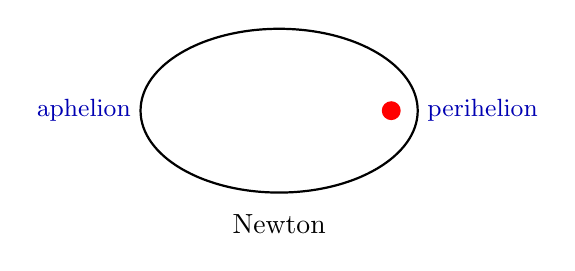
\begin{tikzpicture}[scale=0.8]
  \draw[thick] (0,0) ellipse (2.2 and 1.3);
  \fill[red] (1.78,0) circle (0.15);
  \node[blue!70!black,right,font=\small] at (2.2,0) {perihelion};
  \node[blue!70!black,left,font=\small] at (-2.2,0) {aphelion};
  \node at (0,-1.8) {Newton};
\end{tikzpicture}
\hspace{1.5cm}
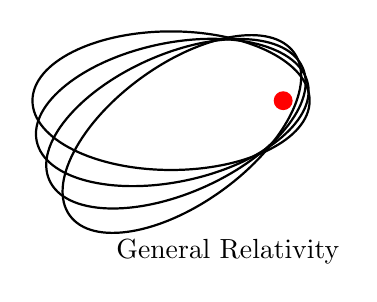
\begin{tikzpicture}[scale=0.8]
  \foreach \a in {0,12,24,36}{\draw[thick,rotate around={\a:(0,0)}] (-0.9,0) ellipse (2.2 and 1.1);}
  \fill[red] (0.88,0) circle (0.15);
  \node at (0,-2.4) {General Relativity};
\end{tikzpicture}
\caption{Left: in Newtonian gravity, a bound orbit is a closed ellipse with the Sun at one focus. Right: in GR the ellipse slowly precesses (the effect is enormously exaggerated here): the perihelion advances at each revolution.}
\label{fig:mercury}
\end{figure}

\section{The classic tests of General Relativity}
\begin{enumerate}[label=(\roman*),nosep]
\item Bending of light (\cref{sec:light-bending}).
\item Precession of the perihelion of Mercury.
\item Shapiro effect (time delay of radar signals passing near the Sun): see Problem Sheet 4, where one finds the maximal delay $\delta t_{\max}=\frac{4\GN M_\odot}{c^3}\big[1+\ln\frac{4r_Ar_B}{R_\odot^2}\big]$.
\item (Gravitational redshift, which already follows from the Equivalence Principle.)
\end{enumerate}
